\section{The BDRF}
\label{sec:bdrf}
Global illumination systems need to describe the radiance from an object, this includes the
reflected radiance by an object from the scene.
The bidirectional reluctance distribution function \cite{Nicodemus65}is a function that describes 
the reluctance of a surface at point $x$ with respect to an outwards direction $\omega_{o}$, and 
inwards direction $\omega_{i}$. The BDRF is commonly written as $f_{r}(x, \omega_{i},\omega_{o})$. 
The BDRF is a vital part of computer graphics as it describes the reluctance of a surface which is 
vital in global illumination as we need to consider reluctance from all objects in a scene.

The BRDF is a me sure of the outgoing radiance $L$ in a given direction $\omega_{o}$ from an incoming
irradiance $E$ from a direction $\omega_{i}$. The BRDF for a surface is given by:

\begin{equation}
f_{r}(\omega_{i}, \omega_{o}) = \frac{L_{\omega_{i}}}{E_{\omega{o}}}
\end{equation}

An example of a simple BDRF would be that of Lambertian reflection whereby the light is reflected
in all directions equally, the BRDF for this is:

\begin{equation}
f_{r}(\omega_{i}, \omega_{o}) = \frac{\rho}{\pi}
\end{equation}

Where $\rho$ is the reflectively of the surface, for physically based rendering this is a real
number between zero and one, the denominator in the expression ensures that the amount of
energy reflected by the surface equals the amount incident on the surface.

\section{The Rendering Equation}
\label{sec:rendering_eq}
First described by Kajiya the rendering equation is an
formulation to the light transfer of a scene \cite{Kajiya86}. A frequency independent version of
the rendering equation is given below:

\begin{equation}
L_{r}(x, \omega_{o}) = L_{e}(x, \omega_{o})
					 +
					   \int_{\Omega}
					 		f_{r}(x, \omega_{i}, \omega_{o})
							L_i(x, \omega_{i})
							(\omega_{i} \cdot n)d\omega_{i}
\end{equation}
where $L_{r}$ is the radiance from the surface at point $x$  in the direction $\omega_o$ ,
$L_{e}$ the emitted radiance from the surface and $f_{r}$
is the BDRF of the surface at $x$ as described in section~\ref{sec:bdrf}.

There have been many developments within computer graphics that attempt to find approximations
to the rendering equation, radiosity \cite{Goral85}which attempts to find the solution by splitting 
the geometry of a scene into smaller patches and builds a system of linear equations that solve the 
radiosity value for the patch, this technique is simple but sufferers from some problems, for one it 
is only able to account for Lambertian diffuse reflections from other object and so cannot be used
to render specular reflections. Radiosity is still used within architectural applications as the
radiometry is view independent and as such is well suited to applications such as walk-throughs.
Monte-carlo methods are another method that is more general that radiometry, this method is a
stochastic method that attempts to find the solution of the rendering equation by sampling the light
transfer of a point until a adequate approximation is found, a common form of this is distributed
ray-tracing whereby ray-tracing as introduced by Whitted \cite{whitted79a} is performed but for each
intersection the choice of reflecting, refracting or absorbing is taken from a distribution as the
number of rays emitted increases the image converges to the solution of the rendering equation.

Understanding the motivations behind the development of the rendering equation will be vital if we are to be successfully in
developing a photon mapping system, the solution that most rendering algorithms produce are an
approximation to the rendering equation and as such will be the focus of my system.

\subsection{Monte Carlo Methods}
The rendering equation describes the light transfer as an integral of all directions above the point being evaluated, this
integral cannot be solved with a closed form solution, as a result we must approximate the value of the integral, to do this
we use monte-carlo methods \cite{wood-monte-carlo}. Monte carlo methods allow us to estimate the value of an integral at a point.
Given a function $f(x)$ which we would like to integrate over the range $[a, b]$

\begin{equation}
I = \int_a^b f(x) dx
\end{equation}

we can form a monte-carlo estimate $I_m$ by taking the average of $N$ uniform samples $\xi_0 ... \xi_n$ over the range $[a, b]$

\begin{equation}
I_m = (b - a) \frac{1}{N} \sum_{i=1}^N f(\xi_i)
\end{equation}

it can be shown that as N tends to infinity our estimator converges to $I$

\[ \lim_{N \to \infty} I_m = I \]

\subsubsection{An Example}
To illustrate the use of monte-carlo method we shall use it to approximate the well known value $\pi$, to do this we
take $n$ samples $(\xi_0, \xi_1)$ on a square with area 4, we then calculate the ratio c / m where c is the number of samples
where $\xi_0^2 + \xi_1^2 <= 1$ , this will approximate the area of the square and a circle with radius 1 which has closed form
solution $\pi / 4$, as we increase the number of samples we approach this value, this can be seen in Figure~\ref{fig:monte-carlo-pi}.

\begin{figure}[h]
	\centering
	\begin{subfigure}{0.45\textwidth}
		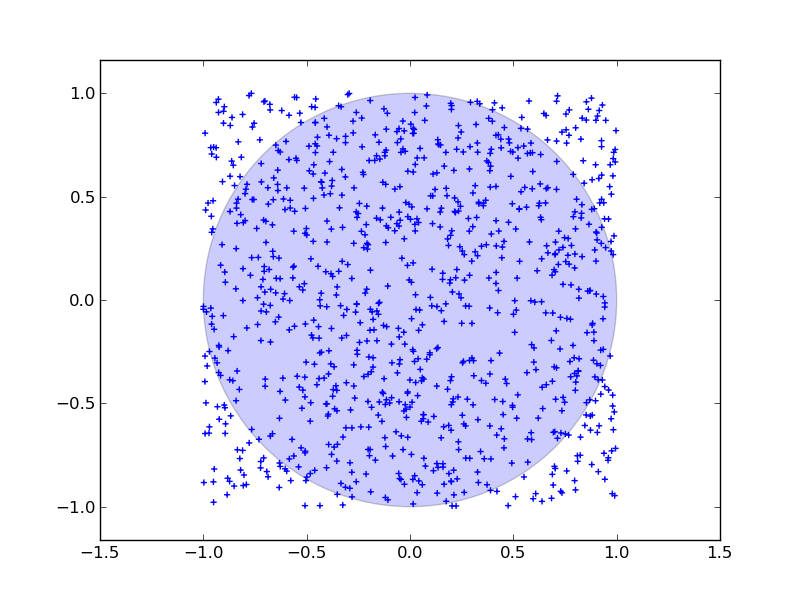
\includegraphics[width=\textwidth]{./images/circle.png}
		\caption{Samples for the simulation}
	\end{subfigure}
	\begin{subfigure}{0.45\textwidth}
		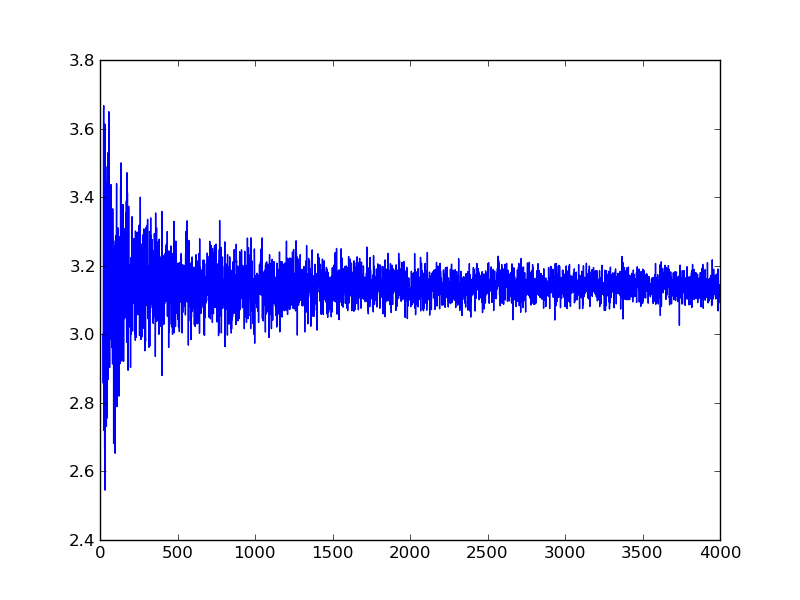
\includegraphics[width=\textwidth]{./images/converge.png}
	\caption{Convergence as $n$ increases}
	\end{subfigure}
	\caption{Monte Carlo simulation to approximate $\pi$}
	\label{fig:monte-carlo-pi}
\end{figure}

%\subsection{Sampling}
%The integral introduced in Section~\ref{sec:rendering_eq} requires us to consider all incoming directions, using monte carlo
%methods we can approximate this integral, this required us to sample the upper hemisphere to generate the samples used
%in the monte carlo evalulation.
%
%\subsubsection{Importance Sampling}
%Importance sampling is a statistical technique that allows us to concentrate computational effort when sampling a distribution
%to areas of the distribution that contribute most to the average, for instance sampling incident radiance at a point on a lambertian
%surface where the reflected radiance is preportional to the cosine of the incoming direction, by using a cosine weighted distribution
%we can gain a better estimate for the radiance.

%\todo{Optional : re-add Importance sampling and extend it}

\section{Ray-tracing}
Ray-tracing is a technique with early developments by Appel \cite{Appel68} and improvements by Whitted \cite{whitted79a} that aims to produce images from scene descriptions that mimics the way
in which light acts, ray are emitted from a virtual eye into a scene and the closest intersection with the ray in the scene is
found, the algorithm then calculates the colour of the object at the point of intersection, this may include refractive or
reflective materials that require additional rays to be traced through the scene, this is called recursive ray-tracing, certain effects can be simulated well with this technique such as shadows which are formed by checking the visibility
of the point of intersection with the light sources in the scene, if the light is blocked by an object in the scene
the object does not receive light from that light source.
